\lecture{16}{29. October 2025}{Boundary Layer Theory}

\section{External Incompressible Viscous Flow}

\subsection{The Boundary Layer Concept}
The boundary layer as a concept was first introduced by Ludwig Prandtl in 1904.
In many ways this served as the \textit{common ground} between the Euler-based field of theoretical hydrodynamics, which predicted no drag and contradicted experiments in many cases, and the empirical field of \textit{hydraulics} which was derived solely from experimental measurements.

The complete equations for viscous flow of a fluid -- the Navier-Stokes equations -- were already known prior to Prandtl, however these equations are impossible to solve analytically except in the simplest cases, prohibiting major theoretical results for viscous flow.
Using Prandtl's idea of a boundary layer, it is possible to analyze many viscous flows by breaking these into two regions, one close to the boundary and one covering the rest of the fluid.
Only in the (relatively) thin \textit{boundary layer} closest to the boundary the effects of viscosity are important.
In the bulk of the fluid (the non-boundary layer region) viscous effects are negligible and the fluid may thus often be treated as inviscid in this area.

In the boundary layer, both viscous and inertial forces are important.
Consequently, the Reynolds-number is important when characterizing boundary-layer flows.
The characteristic length used in the Reynolds number is either the length in the flow direction over which the boundary layer has developed or some measure of the boundary-layer thickness.

Flow in the boundary layer may either be laminar or turbulent.
However, there is no unique value of the Reynolds number for which a transition from laminar to turbulent flow definitively happens in a boundary layer.
Factors such as pressure gradient, surface roughness, heat transfer, body forces, and freestream disturbances also influence when this transition happen.

Often, in real flows, the boundary layer develops over a long, essentially flat surface.
This is a relatively simple flow case as the flow velocity $U$ outside the boundary layer is constant, and therefore this region is steady, inviscid, and incompressible, meaning the pressure will also be constant here.
This constant pressure is the pressure felt by the boundary layer.
This is also known as a \textit{zero pressure gradient flow}.

\begin{figure} [ht]
  \centering
  
\includegraphics[width=0.8\linewidth]{./figures/f9_2.png}
  \caption{Boundary layer on a flat plate.}
  \label{fig:f9_2}
\end{figure}

On \Cref{fig:f9_2} a qualitative picture of the growth of the boundary layer over a flat plate is shown.
Here, it can be seen, that the boundary layer will be laminar for a short distance downstream from the leading edge; then, a transition will occur over a region before the flow turns fully turbulent.

For incompressible flow over a smooth plate with zero pressure gradient, in the absence of heat transfer, with negligible external disturbances this transition can be delayed until the Reynolds number, $\mathrm{Re}_x = \rho U x / \mu$ exceeds \num{e6}. 
For calculation purposes, under typical conditions, transition usually occurs at a length Reynolds number of \num{5e5}.
For air at standard conditions with free stream velocity $U = \qty{30}{\m\per\s}$, this corresponds to $x \approx \qty{0,24}{\m}$.

As the boundary layer is defined as the area where viscous forces are present, as opposed to the free stream, where viscous forces are negligible, it is not unambiguous exactly where the border between the two regions is drawn.
Also, as (in the mathematically idealized situation shown on \Cref{fig:f9_2}) the velocity as a function of distance from the boundary layer will asymptotically approach the free stream velocity, the boundary layer cannot simply be defined as stopping at the point where the local velocity equals the free stream velocity $u = U$.
Therefore, \href{https://xkcd.com/927/}{several different standards are in use} such as: the boundary layer thickness $\delta$, the displacement thickness $\delta^{*}$, and the momentum thickness $\theta$.
These are all shown in comparison on \Cref{fig:f9_3}.

\begin{figure} [ht]
  \begin{subfigure}{0.23\linewidth}
    \centering
    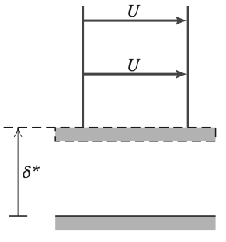
\includegraphics[width=\linewidth]{./figures/f9_3a.png}
    \caption{Displacement thickness, $\delta^{*}$}  
  \end{subfigure}
  \begin{subfigure}{0.15\linewidth}
    \centering
    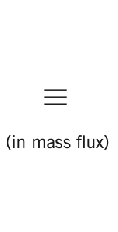
\includegraphics[width=\linewidth]{./figures/f9_3ab.png}
  \end{subfigure}
  \begin{subfigure}{0.23\linewidth}
    \centering
    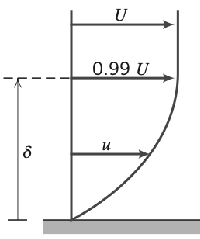
\includegraphics[width=\linewidth]{./figures/f9_3b.png}
    \caption{Disturbance thickness, $\delta$}  
  \end{subfigure}
  \begin{subfigure}{0.13\linewidth}
    \centering
    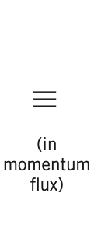
\includegraphics[width=\linewidth]{./figures/f9_3bc.png}
  \end{subfigure}
  \begin{subfigure}{0.23\linewidth}
    \centering
    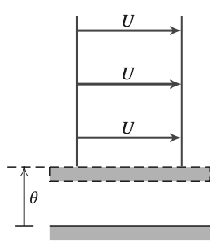
\includegraphics[width=\linewidth]{./figures/f9_3c.png}
    \caption{Momentum thickness, $\theta$}  
  \end{subfigure}
  \caption{Comparison between the different standards for boundary-layer thickness.}
  \label{fig:f9_3}
\end{figure}

The most straightforward of these is the boundary layer thickness, $\delta$.
This is usually defined as the distance from the surface at which the difference between the velocity and the free stream velocity is within 1\%, $u = \num{0,99} U$.

The other two definitions both rely on the fact that the boundary layer slows the fluid, such that the mass flux and momentum flux are both less than they would be without the boundary layer present.

The displacement thickness, $\delta^{*}$, is the distance the plate would be moved such that the loss of mass flux due to the reduction in flow area is equivalent to the loss the boundary layer causes.
For incompressible flow this is:
\[ 
\delta^{*} = \int_{0}^{\infty} 1 - \frac{u}{U} \, \mathrm{d}y \approx \int_{0}^{\delta} 1 - \frac{u}{U} \, \mathrm{d}y 
.\]

The momentum thickness, $\theta$, is the distance the plate would have to be moved such that the loss of momentum flux is equivalent to the loss the boundary layer causes.
This is given as:
\[ 
\theta = \int_{0}^{\infty} \frac{u}{U} \left( 1 - \frac{u}{U} \right) \, \mathrm{d}y \approx \int_{0}^{\delta} \frac{u}{U} \left( 1 - \frac{u}{U} \right) \, \mathrm{d}y 
.\]

The displacement and momentum thickness, $\delta^{*}$ and $\theta$, are easier to evaluate experimentally than the boundary layer thickness $\delta$.


\subsection{Laminar Flat Plate Boundary Layer: Exact Solution}
For two-dimensional, steady, incompressible flow with zero pressure gradient the equations of motion reduces to:
\begin{align*}
\frac{\partial u}{\partial x} + \frac{\partial v}{\partial y} &= 0 \\
u \frac{\partial u}{\partial x} + v \frac{\partial u}{\partial y} &= v \frac{\partial ^2 u}{\partial y^2} 
\end{align*}
with the boundary conditions
\begin{align*}
  u(0) &= 0 & v(0) &= 0 \\
  u(\infty) &= U & \frac{\partial u}{\partial y}(\infty) &= 0
.\end{align*}
These constitute a set of nonlinear, coupled, PDE's for the unknown velocity field $u$ and $v$.
In 1908, H. Blasius showed that the solution to these is of the form
\[ 
  \frac{u}{U} = g(\eta) \quad \text{where} \quad \eta \propto \frac{y}{\delta}
.\]
Further, Blasius reasoned that $\delta \propto \sqrt{vx / U}$ and got
\begin{equation} \label{eq:97}
  \eta = y \sqrt{\frac{U}{vx}}
\end{equation}
The variable $\eta$ combines the variables $x$ and $y$ into one variable.
Using the stream function one can define the function
\[ 
f(\eta) = \frac{\psi}{\sqrt{vxU}}
.\]
The exact solution will not be given in these notes as it is not expected that the derivation will be relevant on an exam.
The solution of this in terms of $\eta$ is shown on \Cref{fig:f9_1}.
From \Cref{fig:f9_1} we see that at $\eta = \num{5,0}$, $u / U \approx \num{0,99}$.
Therefore from \Cref{eq:97} we get:
\[ 
\delta \approx \frac{\num{5,0} }{\sqrt{\frac{U}{vx}}} = \frac{\num{5,0} x}{\sqrt{\mathrm{Re}_x}}
.\]

\begin{figure} [ht]
  \centering
  
\includegraphics[width=0.8\linewidth]{./figures/f9_1.png}
  \caption{The function $f(\eta)$ for the Laminar Boundary Layer along a flat plate at Zero incidence.}
  \label{fig:f9_1}
\end{figure}

The wall shear stress is:
\[ 
\tau_w = \num{0,332} U \sqrt{\rho \mu \frac{U}{x}} = \frac{\num{0,332} \rho U^2}{\sqrt{\mathrm{Re}_x}}
\]
and the wall shear stress coefficient, $C_f$, is given by
\begin{equation} \label{eq:shearstressflatplate}
 C_f = \frac{\tau_w}{\frac{1}{2} \rho U^2} = \frac{\num{0,664}}{\sqrt{\mathrm{Re}_x}}
.\end{equation}

\subsection{Momentum Integral Equation}
We consider the situation of an incompressible, steady, two-dimensional flow over a solid surface.
The boundary-layer thickness, $\delta$, grows with increasing distance, $x$.
We choose a differential control volume of length $\mathrm{d}x$, width $w$, and height $\delta(x)$, as shown in \Cref{fig:f9_4}.
The free stream velocity is denoted $U(x)$.

\begin{figure} [ht]
  \centering
  
\includegraphics[width=0.7\linewidth]{./figures/f9_4.png}
  \caption{Differential control volume in a boundary layer.}
  \label{fig:f9_4}
\end{figure}

We will seek to determine the boundary-layer thickness and shear stress as functions of $x$.
There will be mass flow across surfaces $ab$ and $cd$ of volume $abcd$.
As surface $bc$ is not a streamline but the \textit{imaginary} boundary separating the boundary layer from the free stream there will also be mass flow across $bc$.
As $ad$ constitutes a solid boundary no mass flow will exist across this boundary.
Using the continuity equation for steady flow we start by determining the mass flux through each portion of the control surface.
\[ 
\int _{\mathrm{CS}} \rho \Vec{V} \cdot \mathrm{d}\Vec{A} = 0
.\]
Hence
\[ 
\dot{m}_{ab} + \dot{m}_{bc} + \dot{m}_{cd} = 0 \quad \implies \quad \dot{m}_{bc} = - (\dot{m}_{ab} + \dot{m}_{cd} )
.\]

The mass flux through $ab$ is simply
\[ 
\dot{m}_{ab} = - \left( \int_{0}^{\delta} \rho u \, \mathrm{d}y  \right)w
.\]

Using a Taylor-series expansion the mass flux through $cd$ can be determined to be
\[ 
\dot{m}_{cd} = \left( \int_{0}^{\delta} \rho u \, \mathrm{d}y + \frac{\partial }{\partial x} \left( \int_{0}^{\delta} \rho u \, \mathrm{d}y  \right) \, \mathrm{d}x  \right)
.\]

Thus for surface $\dot{m}_{bc}$ using the above results and the continuity equation we get:
\[ 
\dot{m}_{bc} = - \left( \frac{\partial }{\partial x} \left( \int_{0}^{\delta} \rho u \, \mathrm{d}y  \right)\, \mathrm{d}x  \right) w
.\]

Now we will apply the Momentum equation to the control volume $abcd$, remembering that the flow is steady and under the assumption that body forces are negligible.

We get:
\[ 
\left( F_S \right)_x = \mathrm{mf}_{ab} + \mathrm{mf}_{bc} + \mathrm{mf}_{cd}
\]
where $\mathrm{mf}$ represents the $x$ component of momentum flux.

Once again, we consider the momentum flux over each surface separately.
For surface $ab$ we simply get
\[ 
\mathrm{mf}_{ab} = - \left( \int_{0}^{\delta} u \rho u \, \mathrm{d}y  \right)w
.\]

Using a Taylor series about $x$ we get the momentum flux through $cd$ $\mathrm{mf}_{cd}$ as
\[ 
\mathrm{mf}_{cd} = \left( \int_{0}^{\delta} u \rho u \, \mathrm{d}y  + \frac{\partial }{\partial x} \left( \int_{0}^{\delta} u \rho u \, \mathrm{d}y  \right) \, \mathrm{d}x  \right)w
.\]

Since the mass crossing surface $bc$ has velocity component $U$ in the $x$ direction, the $x$ momentum flux across $bc$ is
\begin{align*}
  \mathrm{mf}_{bc} &= U \dot{m}_{bc} \\
  \mathrm{mf}_{bc} &= - U \left( \frac{\partial }{\partial x} \left( \int_{0}^{\delta} \rho u \, \mathrm{d}y  \right)\, \mathrm{d}x  \right)w
.\end{align*}

Using these we can calculate the net $x$ momentum flux through the control surface as:
\[ 
\int_{\mathrm{CS}} u \rho \Vec{V} \cdot \mathrm{d}\Vec{A} = \left( \frac{\partial }{\partial x} \left( \int_{0}^{\delta} u \rho u \, \mathrm{d}y  \right) \, \mathrm{d}x  - U \frac{\partial }{\partial x} \left( \int_{0}^{\delta} \rho u \, \mathrm{d}y  \right)\, \mathrm{d}x  \right)w
.\]

Now we have an expression for the momentum flux in the $x$ direction through the control surface and we therefore simply need to find expressions for the surface forces acting on the control volume.
Note that $ab$, $bc$, and $cd$ all experience normal forces (i.e. pressure) that generates a force in the $x$ direction. 
In addition, a shear force acts on $ad$.
Since the velocity gradient goes to zero at the edge of the boundary layer, the shear force acting along surface $bc$ is negligible.

If the pressure at $x$ is $p$, then the force acting on $ab$ is
\[ 
F_{ab} = p w \delta
.\]
Due to the small size of the boundary layer it is assumed that $p = p(x)$ within the boundary layer.

Using a Taylor series the force on $cd$ is found to be
\[ 
  F_{cd} = - \left( p + \frac{\partial p}{\partial x} \Bigg]_x \, \mathrm{d}x  \right) w \left( \delta + \mathrm{\delta}  \right)
.\]

The force on $bc$ is
\[ 
F_{bc} = \left( p + \frac{1}{2}  \frac{\partial p}{\partial x} \Bigg]_x \, \mathrm{d}x  \right)w \, \mathrm{d}\delta
.\]

The shear force acting on $ad$ is
\[ 
F_{ad} = - \left( \tau_w + \frac{1}{2} \, \mathrm{d}\tau_w \right)w \, \mathrm{d}x 
.\]

Summing these we obtain the total force acting in the $x$ direction on the control volume
\[ 
  \left( F_S \right)_x \left( - \frac{\partial p}{\partial x} \delta \, \mathrm{d}x - \frac{1}{2} \frac{\partial p}{\partial x} \, \mathrm{d}x \, \mathrm{d}\delta - \tau_w \, \mathrm{d}x - \frac{1}{2} \, \mathrm{d}\tau_w \, \mathrm{d}x  \right) w
.\]
As $\mathrm{d}x  \, \mathrm{d}\delta \ll \delta \, \mathrm{d}x $ and $\mathrm{d}\tau_w \ll \tau_w$ we can neglect the second and fourth terms, leaving us with:
\[ 
\left( F_S \right)_x = \left( - \frac{\partial p}{\partial x} \delta \, \mathrm{d}x  - \tau_w \, \mathrm{d}x  \right)w
.\]

Now substituting these expressions for $\int_{\mathrm{CS}} u \rho \Vec{V} \cdot \mathrm{d}\Vec{A}$   and $\left( F_S \right)_x$ into the momentum equation we obtain
\[ 
\left( - \frac{\partial p}{\partial x} \delta \, \mathrm{d}x - \tau_w \, \mathrm{d}x  \right)w = \left( \frac{\partial }{\partial x} \left( \int_{0}^{\delta} u \rho u \, \mathrm{d}y  \right)\, \mathrm{d}x - U \frac{\partial }{\partial x} \left( \int_{0}^{\delta} \rho u \, \mathrm{d}y  \right)\, \mathrm{d}x  \right)w
.\]
Dividing this by $w \, \mathrm{d}x $ gives
\[ 
- \delta \frac{\partial p}{\partial x} - \tau_w = \frac{\partial }{\partial x} \int_{0}^{\delta} u \rho u \, \mathrm{d}y - U \frac{\partial }{\partial x} \int_{0}^{\delta} \rho u \, \mathrm{d}y
.\]
The above can be rewritten as
\[ 
\tau_w = - \frac{\partial }{\partial x} \int_{0}^{\delta} u \rho u \, \mathrm{d}y + U \frac{\partial }{\partial x} \int_{0}^{\delta} \rho u \, \mathrm{d}y + \frac{\mathrm{d}U}{\mathrm{d}x} \int_{0}^{\delta} \rho U \, \mathrm{d}y 
.\]

Or, rewriting further and using the definitions of displacement thickness $\delta^{*}$ and momentum thickness $\theta$, we obtain:
\begin{equation} \label{eq:mominteq}
  \frac{\tau_w}{\rho} = \frac{\mathrm{d}}{\mathrm{d}x} \left( U^2 \theta \right) + \delta^{*}U \frac{\mathrm{d}U}{\mathrm{d}x} 
\end{equation}
\Cref{eq:mominteq} is known as the \textit{momentum integral equation} and is restricted to a steady incompressible two-dimensional flow.
This will yield an ODE for boundary-layer thickness $\delta$ as a function of $x$.


\subsection{Use of the Momentum Integral Equation for Flow with Zero Pressure Gradient} \label{sec:flatplate}
For the special case of a flat plate (i.e. zero pressure gradient) the free stream pressure $p$ and velocity $U$ are both constant.

The momentum integral equation then reduces to
\[ 
\tau_w = \rho U^2 \frac{\mathrm{d}\theta}{\mathrm{d}x} = \rho U^2 \frac{\mathrm{d}}{\mathrm{d}x} \int_{0}^{\delta} \frac{u}{U} \left( 1 - \frac{u}{U} \right)\, \mathrm{d}y 
.\]
Here, the velocity distribution $u / U$ in the boundary layer is assumed to be similar for all $x$ and is normally given as a function of $y / \delta$.
For this reason it is convenient to change the variable of integration from $y$ to $y / \delta$.
By defining
\[ 
\eta = \frac{y}{\delta}
\]
we get
\[ 
\mathrm{d}y = \delta \, \mathrm{d}\eta
\]
and the momentum integral equation for zero pressure gradient is written
\[ 
\tau_w = \rho U^2 \frac{\mathrm{d}\theta}{\mathrm{d}x} = \rho U^2 \frac{\mathrm{d}\delta}{\mathrm{d}x} \int_{0}^{1} \frac{u}{U} \left( 1 - \frac{u}{U} \right)\, \mathrm{d}\eta
.\]

To solve this equation for the boundary layer thickness as a function of $x$ we first assume a velocity distribution in the boundary layer of the form
\[ 
\frac{u}{U} = f \left( \frac{y}{\delta} \right)
.\]
The assumed velocity distribution should satisfy the boundary conditions:
\begin{align*}
  u(0) &= 0 \\
  u(\delta) &= U \\
  \frac{\mathrm{d}u}{\mathrm{d}y} (\delta) &= 0
.\end{align*}
Once a velocity distribution is assumed the integral in the equation from before reduces to:
\[ 
\int_{0}^{1} \frac{u}{U} \left( 1 - \frac{u}{U} \right)\, \mathrm{d}\eta = \frac{\eta}{\delta} = \mathrm{constant} = \beta
\]
and the momentum integral equation becomes
\[ 
\tau_w = \rho U^2 \frac{\mathrm{d}\delta}{\mathrm{d}x} \beta
,\]
which is an expression for $\tau_w$ in terms of $\delta$.
This can be used to solve for $\delta(x)$.

\paragraph{Laminar Flow}
For laminar flow over a flat plate, it turns out that a reasonable assumption for the velocity profile is a polynomial in $y$:
\[ 
u = a + by + cy^2
.\]
Evaluating constants $a$, $b$, and $c$ given the boundary conditions we obtain:
\[ 
\frac{u}{U} = 2 \left( \frac{y}{\delta} \right) - \left( \frac{y}{\delta} \right)^2 = 2 \eta - \eta^2
.\]
The wall shear stress is given by:
\[ 
\tau_w = \mu \frac{\partial u}{\partial y} \Bigg)_{y = 0}
.\]
Substituting the assumed velocity profile into this we get:
\[ 
\tau_w = \mu \frac{\partial u}{\partial y} \Bigg]_{y = 0} = \mu \frac{U \partial \frac{u}{U}}{\delta \partial \frac{y}{\delta}}_{\frac{y}{\delta} = 0} = \frac{\mu U}{\delta} \frac{\mathrm{d}\frac{u}{U}}{\mathrm{d}\eta} \Bigg]_{\eta = 0}
\]
or
\[ 
\tau_w = \frac{\mu U }{\delta} \frac{\mathrm{d}}{\mathrm{d}\eta} \left( 2 \eta - \eta^2 \right) \Bigg]_{\eta = 0} = \frac{\mu U }{\delta} \left( 2 - 2\eta \right) \Bigg]_{\eta = 0} = \frac{2\mu U}{\delta}
.\]
This shows that the wall stress $\tau_w$ is a function of $x$, since the boundary layer thickness $\delta = \delta(x)$.

Substituting for $\tau_w$ and $u / U$ into the momentum integral equation \Cref{eq:mominteq}, we obtain
\[ 
\frac{2\mu U}{\delta} = \rho U^2 \frac{\mathrm{d}\delta}{\mathrm{d}x} \int_{0}^{1} \left( 2\eta - \eta^2 \right) \left( 1 - 2\eta + \eta^2 \right)\, \mathrm{d}\eta
\]
or
\[ 
\frac{2 \mu U}{\delta \rho U^2} = \frac{\mathrm{d}\delta}{\mathrm{d}x} \int_{0}^{1} \left( 2 \eta - 5 \eta^2 + 4 \eta^3 - \eta^{4} \right)\, \mathrm{d}\eta
.\]
Integrating this and substituting limits yields
\[ 
\frac{2\mu}{\delta \rho U} = \frac{2}{15} \frac{\mathrm{d}\delta}{\mathrm{d}x} \quad \text{or} \quad \delta \, \mathrm{d}\delta = \frac{15\mu}{\rho U}\, \mathrm{d}x 
\]
which is a differential equation for $\delta$.
Integrating again yields
\[ 
\frac{\delta^2}{2} = \frac{15\mu}{\rho U }x + c
.\]
We assume $\delta = 0$ at $x = 0$, meaning $c = 0$ and thus
\[ 
\delta = \sqrt{\frac{30\mu x}{\rho U}}
.\]
This shows that a laminar boundary layer will grow in thickness $\delta$ with $\sqrt{x}$; i.e. it has a parabolic shape.
Traditionally this is expressed in dimensionless form:
\[ 
\frac{\delta}{x} = \sqrt{\frac{30\mu}{\rho U x}} = \frac{\num{5,48} }{\sqrt{\mathrm{Re}_x}}
.\]
I.e. the ratio of boundary layer thickness to distance along a flat plate varies inversely with the square root of length Reynolds number.

The wall shear stress, or ``skin friction'' coefficient is defined as:
\[ 
C_f \equiv \frac{\tau_w}{\frac{1}{2}\rho U^2}
.\]

Substituting in the velocity profile and the equation for $\delta / x$ we get:
\[ 
C_f = \frac{\tau_w}{\frac{1}{2}\rho U^2} = \frac{2 \mu \frac{U}{\delta}}{\frac{1}{2} \rho U^2} = \frac{4 \mu}{\rho U \delta} = \frac{\num{0,730} }{\sqrt{\mathrm{Re}_x}}
.\]


\paragraph{Turbulent Flow}
For the flat plate, we still have $U = \text{constant}$.
We must, once again, start by approximating the velocity profile and an expression for $\tau_w$.
The turbulent velocity profile is often assumed to be
\[ 
\frac{u}{U} = \left( \frac{y}{\delta} \right)^{\frac{1}{7}} = \eta^{\frac{1}{7}}
.\]
However, this does not hold right next to the wall as it predicts $\mathrm{d}u / \mathrm{d}y (0) = \infty$.
Consequently, it cannot be used to define $\tau_w$.
We therefore adapt the expression for pipe flow to:
\[ 
\tau_w = \num{0,0332} \rho \overline{V}^2 \left( \frac{\nu}{R \overline{V}} \right)^{\num{0,25} }
.\]
For a $1 / 7$-power profile in a pipe, $\overline{V} / U = \num{0,817}$.
Substituting this and $R = \delta$ into the above we get
\[ 
\tau_w = \num{0,0233} \rho U^2 \left( \frac{\nu}{U \delta} \right)^{\frac{1}{4}}
.\]
Substituting this into \Cref{eq:mominteq} we get:
\[ 
\num{0,0233}  \left( \frac{\nu}{U \delta} \right)^{\frac{1}{4}} = \frac{\mathrm{d}\delta}{\mathrm{d}x} \int_{0}^{1} \eta^{\frac{1}{7}} \left( 1 - \eta^{\frac{1}{7}} \right)\, \mathrm{d}\eta = \frac{7}{72} \frac{\mathrm{d}\delta}{\mathrm{d}x} 
.\]
This gives a differential equation for $\delta$:
\[ 
\delta^{\frac{1}{4}} \, \mathrm{d}\delta = \num{0,240}  \left( \frac{\nu}{U} \right)^{\frac{1}{4}} \, \mathrm{d}x 
.\]
By integration we get:
\[ 
\frac{4}{5} \delta^{\frac{5}{4}} = \num{0,240} \left( \frac{\nu}{U} \right)^{\frac{1}{4}} x + c
.\]
We assume that $\delta \approx 0$ at $x = 0$, meaning the flow is assumed turbulent from the leading edge, then $c = 0$ and
\[ 
\delta = \num{0,382} \left( \frac{\nu}{U} \right)^{\frac{1}{5}} x^{\frac{4}{5}}
.\]
This shows that the turbulent boundary layer thickness $\delta$ grows as $x^{\frac{4}{5}}$.
In dimensionless form this is:
\[ 
\frac{\delta}{x} = \num{0,382} \left( \frac{\nu}{Ux} \right)^{\frac{1}{5}} = \frac{\num{0,382} }{\mathrm{Re}_x^{\frac{1}{5}}}
.\]

And the skin friction coefficient is:
\begin{equation} \label{eq:turbskinfric}
  C_f = \frac{\tau_w}{\frac{1}{2}\rho U^2} = \frac{\num{0,0594} }{\mathrm{Re}_x^{\frac{1}{5}}}
\end{equation}
Experiments show that \Cref{eq:turbskinfric} is fairly accurate for $\num{5e5} < \mathrm{Re}_x < \num{e7}$.


\subsection{Pressure Gradients in Boundary Layer Flow}
For all bodies, except a flat plate as previously studied, a pressure gradient will be present.

A \textit{favorable pressure gradient} is one in which the pressure decreases in the flow direction ($\partial p / \partial x < 0$).
This tends to work to overcome friction-caused slowing in the boundary layer.
On the other hand, an \textit{adverse pressure gradient} is one in which pressure increases in the flow direction ($\partial p / \partial x > 0$). 
If an adverse pressure gradient is severe enough, the fluid particles in the boundary layer will be brought to rest.
When this occurs, the particles will be forces away from the body surface (a phenomenon called \textit{flow separation}), which leads to a turbulent wake.

For uniform flow over a flat plate, the flow \textit{never} separates and we never develop a wake region, whether the boundary layer is laminar or turbulent, regardless of plate length.

For favorable pressure gradients we will also never observe flow separation.
Furthermore, an adverse pressure gradient does not \textit{always} lead to flow separation and a wake -- i.e., it is a necessary but not a sufficient condition for flow separation.

